\documentclass[12pt,letterpaper]{article}
\usepackage{fullpage}
\usepackage[top=2cm, bottom=4cm, left=2cm, right=2cm]{geometry}
\usepackage{amsmath,amsthm,amsfonts,amssymb,amscd}
\usepackage{lastpage}
\usepackage{enumerate}
\usepackage{fancyhdr}
\usepackage{mathrsfs}
\usepackage{xcolor}
\usepackage{graphicx}
\usepackage{listings}
\usepackage{hyperref}
\usepackage{siunitx}
\usepackage{appendix}
\usepackage{caption}
\usepackage{subcaption}

\hypersetup{%
  colorlinks=true,
  linkcolor=blue,
  linkbordercolor={0 0 1}
}
 
\renewcommand\lstlistingname{Algorithm}
\renewcommand\lstlistlistingname{Algorithms}
\def\lstlistingautorefname{Alg.}

\lstdefinestyle{Python}{
    language        = Python,
    frame           = lines, 
    basicstyle      = \footnotesize,
    keywordstyle    = \color{blue},
    stringstyle     = \color{green},
    commentstyle    = \color{orange}\ttfamily
}

\setlength{\parindent}{0.0in}
\setlength{\parskip}{0.05in}

% Edit these as appropriate
\newcommand\course{ASTRO 372}
\newcommand\coursename{Computational Methods for Physics}
\newcommand\hwnumber{1}                  % <-- homework number
\newcommand\myname{Sandra Bustamante}           % <-- NetID of person #1
%\newcommand\NetIDb{netid12038}           % <-- NetID of person #2 (Comment this line out for problem sets)

\pagestyle{fancyplain}
\headheight 35pt
\lhead{\coursename\\\course}
\chead{\textbf{\Large Homework \hwnumber}}
\rhead{\myname \\ \today}
\lfoot{}
\cfoot{}
\rfoot{\small\thepage}
\headsep 1.5em

%%%%%%%%%%%%%%%%%%%%%%%%%%%%%%%%%%%%%%%%%%%%%%%%%%%%%%%%%%%%%%%
%=====================BEGIN DOCUMENT===========================
%%%%%%%%%%%%%%%%%%%%%%%%%%%%%%%%%%%%%%%%%%%%%%%%%%%%%%%%%%%%%%%

\begin{document}

%=========PROBLEM 1============================================
\section*{Problem 1}

This problem wants us to learn how to plot a function and making it legible when it needs to be included in \LaTeX documents such as this homework. 

\begin{figure}[t]
    \centering
    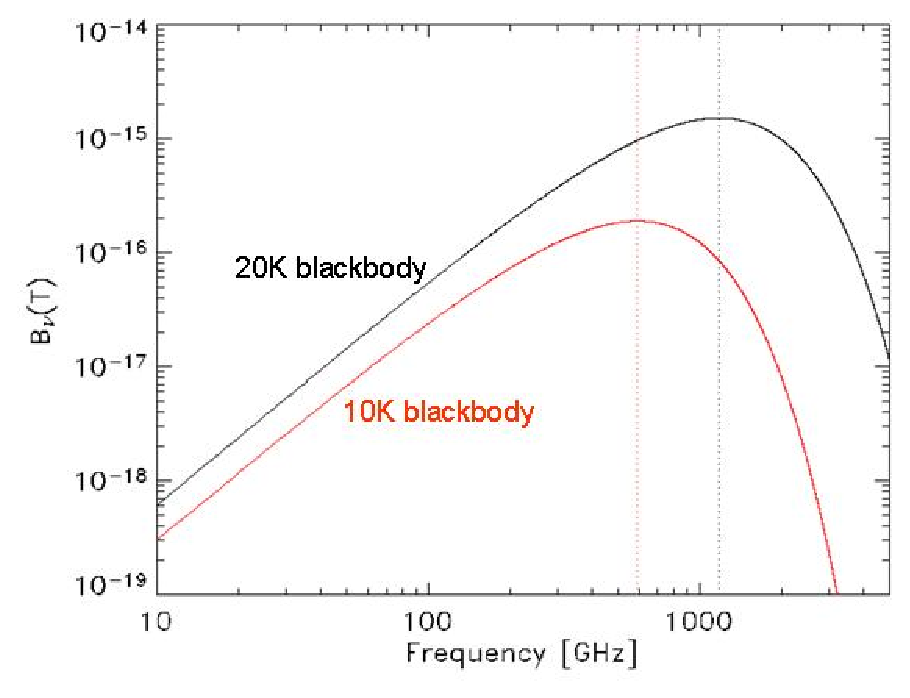
\includegraphics[scale=1]{figures/planck.eps}
    \caption{Original Plot}
    \label{fig:grantOriginalPlot}
\end{figure}

\begin{figure}[t]
    \centering
    \includegraphics[scale=1]{figures/hw01prob1-1.png}
    \caption{Plot created by python code "hw01prob1-1.py"}
    \label{fig:blackbodyRadiationPlot}
\end{figure}

The requirements are:

\begin{itemize}
    \item Axis labels should be readable and correct
    \item Text in plot should be the same size as text in document. \textit{(optional but recommended)}
    \item Plot should accurately show the blackbody radiation of two blackbodies, \SI{10}{\kelvin} and \SI{20}{\kelvin}.
\end{itemize}

The steps followed to recreate this plot were the following:
\begin{enumerate}
    \item \textbf{Look up the constants.}
    
     I look up the current constants on the NIST website which were defined on the 2018 CODATA. To make it easier for the future me, I define a function with my constants which can be updated as needed.
     
    \item \textbf{Determined my variables.}
    
    \item \textbf{Calculate the blackbody radiation and frequency of the peak.}
    
    To calculate the blackbody radiation I used Planck's Law given by,
        \begin{equation}
        B_\nu(T) = \frac{2h\nu^3}{c^2}\frac{1}{e^{h\nu /kT}-1} \mbox{ [Hz]}
        \label{eq:Plancks}
        \end{equation}
    To calculate the maximum frequency I used Wien's Displacement Law given by,
        \begin{equation}
         \nu_{\rm{max}} = 5.879\times 10^{10} T \mbox{ [\si{\hertz}]}
        \label{eq:WienDisp}
        \end{equation}. 
    In the code, these equations are defined as functions.
    
    \item \textbf{Plot my equations.}
    
    To show the blackbody radiation correctly, both the frequency axis and the radiation axis need to be in log form. To do this, I use the loglog command. 
    The maximum frequency is shown as a vertical line, so to achieve this a I use the axvline command.
    
    \item \textbf{Customize the plot to achieve a readable plot.}
    
    To customize the plot I define the following main parameters:
        \begin{itemize}
            \item Font: 8pt
            \item Width: 3.39 for it to show in a single column size or 6.9 for use a double column size. 
            \item Height: 2.41 for a single column or 4.26 for a double column. The height was calculate from the Golden Mean $= \sqrt{5}-1 / 2 $, which is determined to be an aesthetic ratio. 
        \end{itemize}
\end{enumerate}

The final figure produced is shown on Figure  \ref{fig:blackbodyRadiationPlot}.
%=========PROBLEM 2============================================
\section*{Problem 2}

The AzTEC mm-wavelength camera completed a large survey of the COSMOS field in search for sub-millimeter galaxies. 
A typical source detection is between 4 and 10 sigma level. 
Before analyzing the data, is important to understand the noise properties of the camera. 
To do this, noise maps are produced. A noise map is a map with little to no astronomical signal. 
In this problem, a noise map of AzTEC was given. We need to produce two histograms, one linear and another in semi-log form, of the data within the center 20 arc-minutes of the map. 
The pixel size is $3 \times 3$ arc-seconds.

The steps followed to do the histograms are the following:

\begin{enumerate}
    \item Import fits file and read header.
    
    FITS stands for Flexible Image Transport System. It is a standard used mainly in astronomy to save data of the observations in a standard way. To import a fits file into Python so that the data can be accessed, a viewer is needed. It was recommended to use PyFits which was ported to Astropy as "astropy.io.fits". For this reason, astropy was used for this and subsequent problems as needed. 
    
    Once the fits viewer was imported, 
    \lstinline[columns=fixed, style=Python]{fits.open()} 
    will open the fits file. The fits file is compose of a list of objects which are compose of two parts: a header and the data. The header is were the metadata of the image is located. It gives information such as the timestamp, the instrument used, the number of axes, the number of pixels, etc. These parameters can be put into a variable by calling them by their label. 
    
    \item Extract the data of the centered 20 arcminutes.
    
    A mask is used to achieve this step. A mask is a matrix of the same size as the data which contains boolean values. If True, the data will stay as is and if False, the data will be turn into zero. This process will only "make visible" the data we are interested. 
    
    The mask "shape" will be a circle since the information needed is the within 20 arcminutes of the center of the map. Using the header, the location of the central pixel can be estimated by taking the length of the axis and divide it by 2. It is known that the equation of the circle is given by 
    \begin{equation} \label{eq:circle}
        r = \sqrt{(x-x_0)^2 + (y-y_0)^2}
    \end{equation}
    where $x_0$ and $y_0$ are the coordinates of the center and $r$ is the radius of the circle. 
    
    The radius of the circle is 20 arcminutes which transformed into pixels, given that each pixel is 3 arcseconds, is 
    \begin{equation}\label{eq:radiusInPixels}
        r= 20' \times \frac{60''}{1'} \times \frac{1  \mathrm{pixel}}{3''} = 400 \mathrm{pixel}
    \end{equation}
    
    Comparing the right hand of equation \ref{eq:circle} bigger than r in pixels, outputs a boolean array with same dimensions as the data, in other words, it creates the mask. The mask is applied to the data and later trimmed so it will contain the information wanted. 
    
    \item Create histograms.
    
    An histogram shows how many times the values in a range are repeated. The range is given by the bin size. Since the values are being counted, the positions of the values are not important at this point. The \lstinline[columns=fixed, style=Python]{data.flatten()} command makes the 2 dimensional array into a 1 dimensional array. After this, the data is ready to get the histogram. 
    
    The histograms of the values are given by Figure \ref{fig:histograms}. 
    
    \begin{figure}[]
        \centering
        \includegraphics{figures/hw01prob1-2fig1.png}
        \caption{Histograms of the noise map of AzTEC. Top: Histogram in a linear form. Bottom: Histogram in a semi-log form.}
        \label{fig:histograms}
    \end{figure}
    
     \item \textbf{Customize the plot to achieve a readable and understandable plot.}
     
\end{enumerate}

The histogram in its linear form shows a bell-like shape. This shape is associated to a normal distribution or to a Gaussian. The mean of the data will be the center of this shape. This suggests that the noise is produced by a random process.

The histogram in its semilog form shows a more rounded shape.This shows that most values are near the center. 

\include{problem1-3}
%=========PROBLEM 4============================================
\section*{Problem 4}
\label{sec:problem4}
All computers treat numbers as approximation to the nearest bit representation of that number. It will greatly differ by the amount of bits used and the type of number. Numbers that are type \textit{int} are always exact but that is not the case for example to numbers of type \textit{float}. This exercise asks to find the minimum value of $\epsilon$ that will satisfy the following conditions and considering data type of float32 and float64:
\begin{enumerate}
    \item[a)] $1 + \epsilon > 1$
    \item[b)] $1 - \epsilon < 1$
    \item[c)] $10^16 +\epsilon > 10^16$
    \item[d)] $10^16 -\epsilon < 10^16$
\end{enumerate}

The steps to solve this problem are the following:

\begin{enumerate}
    \item Initialize my variables.
    \item Evaluate the condition for the first time and save it as prev\_eps.
    \item Evaluate the condition. 
    \label{item:Init}
    If this condition is different than the previous condition than continue to step \ref{item:DiffTrue}, if not continue to step \ref{item:DiffFalse}.
    \item Calculate the new step, h:
    \label{item:DiffTrue}
        \begin{equation}
            h = \frac{\epsilon_0 - \epsilon_1}{2}
        \end{equation}
    \item Calculate new $\epsilon$ with,
        \label{item:DiffFalse}
        \begin{equation}
            \epsilon_1=\epsilon_0 + h
        \end{equation}
        Then continue to step \ref{item:Init}
    \item 
    
Every iteration across my threshold, I would reduce my step by 2.  
    
\end{enumerate}

Table \ref{tab:epsilon} shows the different values of $\epsilon$ that satisfies the condition using either float32 and float64. In the first two cases, the values are different within each other. This could be because 1 only needs one bit for its representation so the decimals and be stored in the rest of the bits. In the second two cases, the values are equals within each same data type. This could be because $10^{16}$ is so big that float32 doesn't get enough bit space left. 

\begin{table}[]
    \centering
    \begin{tabular}{c|l|l}
        CONDITION            & FLOAT 32 BITS            & FLOAT 64 BITS \\
        $1 + \epsilon > 1$  & $5.960465\times 10^{-08}$ & $1.1102230246251568 \times 10^{-16}$\\
        $1 - \epsilon < 1$ & $2.9802322\times 10^{-08}$ & $5.551115123125783 \times 10^{-17}$ \\
        $10^{16} +\epsilon > 10^{16}$ & $536871000.0$ & $1.0000000000000002$ \\
        $10^{16} -\epsilon < 10^{16}$ & $536871000.0$ & $1.0000000000000002$\\
    \end{tabular}
    \caption{Shows the smallest value of $\epsilon$} that satisfies the condition given at different data type.
    \label{tab:epsilon}
\end{table}
%=========PROBLEM 5============================================
\section*{Problem 5}

All computers treat numbers as approximation to the nearest bit representation of that number. It will greatly differ by the amount of bits used and the type of number. Numbers that are type \textit{int} are always exact but that is not the case for example to numbers of type \textit{float}. In addition, the values between different data types but same operation will differ notably. This is an unstability. This exercise asks to show the unstability of the "Golden Mean Ratio" when using the following equation, 

\begin{equation}
    \phi^{n+1}=\phi^{n-1}-\phi^{n}
\end{equation}

Knowing that $\phi^0=1$ and $\phi^1=\frac{\sqrt{5}-1}{2}$, the previous formula becomes a subtraction of known values. An easier way to see it is that equation becomes "the future value of $\phi$ is equal to the past value - the present value". In this way, if we are on the first iteration, the present value is $\phi^n$ which is a known value and $\phi^{n=1}$ aka the future value is calculated. 

The values of $\phi$ can be seen in Figure \ref{fig:phi}.

\begin{figure}
    \centering
    \includegraphics{figures/hw01prob1-5fig1.png}
    \caption{Top: Shows the values of $\phi$ using the Golden Mean Recursion. Bottom: Shows a zoom so that the differences are more clearly seen.}
    \label{fig:phi}
\end{figure}

\appendix

\lstset{caption={CodeHw01-1.py}, style=Python}

\section[]{Python code to solve Problem 1} 
\label{sec:CodeHw01-1}
\lstset{label={hw01prob1-1.py}}
\lstinputlisting[language=Python]{code/hw01prob1-1.py}

\newpage
\section[]{Python Code to Solve Problem 2} 
\label{sec:CodeHw01-2}
\lstset{label={hw01prob1-2.py}}
\lstinputlisting[language=Python]{code/hw01prob1-2.py}

\newpage
\section[]{Python Code to Solve Problem 3} 
\label{sec:CodeHw01-3}
\lstset{label={hw01prob1-3.py}}
\lstinputlisting[language=Python]{code/hw01prob1-3.py}

\newpage
\section[]{Python Code to Solve Problem 4} 
\label{sec:CodeHw01-4}
\lstset{label={hw01prob1-4v1.py}}
\lstinputlisting[language=Python]{code/hw01prob1-4v1.py}

\newpage
\section[]{Python Code to Solve Problem 5} 
\label{sec:CodeHw01-5}
\lstset{label={hw01prob1-5.py}}
\lstinputlisting[language=Python]{code/hw01prob1-5.py}

\end{document}